\PassOptionsToPackage{hidelinks}{hyperref}

\documentclass[doc,biblatex]{apa7}

\usepackage{amsmath}
\usepackage{mathspec}
\usepackage{fontspec}

\DeclareLanguageMapping{american}{american-apa}
\addbibresource{references.bib}

\captionsetup[figure]{textfont=rm,font=small,labelfont=bf}
\setallmainfonts{Minion Pro}
\setmainfont{Minion Pro}

\newfontfamily\doulos{Doulos SIL}[Scale=MatchLowercase]
\DeclareTextFontCommand\textdoulos{\doulos} % for IPA

\newfontfamily\timesnewroman{Times New Roman}[Scale=MatchLowercase]
\DeclareTextFontCommand\texttimes{\timesnewroman} % for Hebrew

\newcommand\lemma[2]{\textsc{#1·#2}}
\newcommand\spelling[1]{\allowbreak$\langle$#1$\rangle$}
\newcommand\pronunciation[1]{/\textdoulos{#1}/}

\title{Frequency-dependent selection in the English spelling system across 1000 years of history}

\shorttitle{Frequency-dependent selection in the English spelling system}

\authorsnames{Jon W. Carr, Kathleen Rastle}

\authorsaffiliations{{Department of Psychology, Royal Holloway, University of London}}

\authornote{\textbf{Cite as:} Carr, J.\@ W., \& Rastle, K.\@ (2024). Frequency-dependent selection in the English spelling system across 1000 years of history. \textit{PsyArXiv}. Version~1. \url{https://doi.org/10.31234/osf.io/kaqgf}}

\abstract{English orthography has largely been left to evolve freely across its thousand-year history with little top-down design or reform. Yet modern English spelling has become standardized, even if its standardized spellings are sometimes internally inconsistent. The relative freedom with which English orthography has been allowed to evolve makes it an interesting test-case for exploring whether spelling standardization might arise through a process of positive frequency-dependent selection. To maximize the chance of being understood, it pays for a writer to adopt spelling variants that occur with higher frequency, leading to those forms becoming increasingly entrenched. To evaluate this possibility, we assembled a diachronic dataset of English spelling variation, SpellEng, which we make freely available. SpellEng reports on the frequency of 112,080 spelling variants (across 32,264 lemmata) over the entire history of the English language. We use this dataset along with a model of frequency-dependent selection to estimate the extent to which English standardization can be explained by such a process. Our findings suggest that the past 1000 years of English spelling have been characterized by both positive and negative frequency-dependent selection. We discuss how linguistic dynamics and external events have shaped these periods of stability and change.}

\keywords{corpus; English; evolution; frequency-dependent selection; reading; spelling; variation; writing}

\begin{document}

\maketitle

\noindent
English has a rich history of spelling variation. To take one particularly extreme example, the \textit{Oxford English Dictionary} (OED) lists 441 historical spelling variants of the word \textit{through}, including such curiosities as \spelling{thrvoo}, \spelling{yrowȝ}, \spelling{ðerh}, \spelling{þrowghe}, and \spelling{zhorw}, as well as the modern variant spelling \spelling{thru}. Spelling variation is known to have peaked in the Middle English period (c.~1150--1500), a time of great change in the English language. In the 15th century alone, the OED provides quotational evidence for 24 different spellings of the word \textit{little} (e.g., \spelling{litel}, \spelling{littill}, and \spelling{lytul}), a common and relatively unambiguous word on which we might expect there to be broad agreement. It is also widely noted that substantial levels of variation can be found both within the same text \parencite[e.g.,][]{Wojcik:2021} and within the same author \parencite[e.g.,][]{Evans:2012}. Such high levels of variation have been variously attributed to contact with French following the Norman conquest in 1066, the impact of the Great Vowel Shift (c.~1400--1700), and English's status as a set of local spoken vernaculars, rather than a unified language of prestige, for a large part of its history \parencite{Crystal:2005, Fisher:1996, Scragg:1974, Smith:1996, Vallins:1954}.

English is also notable for the relative freedom with which its spelling system has evolved \parencite{Stenroos:2016}. This freedom \parencite[or ``anarchy'' as described by][]{Berg:2017} has resulted in a spelling system that is often viewed as irregular and complex, with numerous exceptions and idiosyncrasies. Historically, the main regularizing forces in English orthography include the emergence of the ``Chancery standard'' in London during the 15th century \parencite{Fisher:1996, Wright:2020}, the introduction of the printing press to England in 1476 and the associated development of various ``house styles'' \parencite{Condorelli:2022}, and the publication of several English dictionaries, such as Mulcaster's \textit{Elementarie} in 1582, Cawdrey's \textit{Table Alphabeticall} in 1604, and Johnson's \textit{Dictionary of the English Language} in 1755 \parencite{Considine:2012}. Nevertheless, English orthography has never been subjected to the kind of systematic reform that occurred in other European languages through language academies. Dutch, German, and Spanish, for example, have undergone several orthographic reforms over the past few centuries \parencite{Baddeley:2012, Neijt:2023, Stickel:2012, Villa:2015}, while proposals for spelling reform in English, such as those of \textcite{Hart:1569} and the \textcite{SSB:2012}, have largely proven unsuccessful \parencite{Zachrisson:1931}.

Despite these two characteristics---high levels of historical variation and a lack of formal regulation---modern English spelling \textit{has} nevertheless become highly standardized, with almost every word having only one permitted spelling. However, unlike the top-down standardization process applied to many other orthographies, the bottom-up standardization of English orthography has resulted in a set of spellings that are often internally inconsistent. To take one example, the diphthong \pronunciation{eɪ} can be spelled at least eight different ways---\spelling{ae} as in \textit{brae}, \spelling{aigh} as in \textit{straight}, \spelling{ai} as in \textit{raid}, \spelling{ay} as in \textit{stay}, \spelling{ea} as in \textit{break}, \spelling{eigh} as in \textit{eight}, \spelling{ei} as in \textit{feign}, and \spelling{ey} as in \textit{they}, not to mention the combinations with final-\spelling{e}, as in \textit{crepe}, \textit{praise}, and \textit{waste} \parencite{Rastle:2002}.

Some of this internal inconsistency may be functional. For example, the fact that there are several possible spellings of word-final \pronunciation{əs} (e.g., \spelling{as} as in \textit{atlas}, \spelling{us} as in \textit{bonus}, \spelling{ose} as in \textit{purpose}) allows for one particular spelling (\spelling{ous}) to be reserved for communicating adjective status (\textit{jealous}, \textit{nervous}, \textit{serious}), allowing the written form of the language to convey more information than its spoken counterpart \parencite{Berg:2017, Rastle:2019, Ulicheva:2020}. Similarly, the heterographic spelling of homophonous words (e.g., \spelling{their}, \spelling{there}, and \spelling{they're}) may serve a useful disambiguating function for readers \parencite{CarrRastle:2024}. It is generally accepted, however, that the relative lack of spelling-sound systematicity in English poses challenges both for learning to read \parencite{Seymour:2003} and for skilled reading \parencite{Glushko:1979}. It is therefore interesting to consider how the informal process of English spelling standardization resulted in a system that appears to be far from optimal for the primary purpose of reading.

In this paper, we consider the possibility that the gradual standardization of English spelling might be explained, at~least partially, through a process of frequency-dependent selection at the level of the word. Frequency-dependent selection---originally a concept from evolutionary biology---refers to a situation where the fitness of a variant depends on its frequency relative to other variants in a population, over and above the inherent fitness of the variant itself \parencite{Svensson:2019}. \textit{Positive} frequency-dependent selection occurs when the fitness of a variant \textit{increases} as it becomes more common in the population, which ultimately tends to lead to the dominance of that variant over others. For example, in species that use colors or patterns to ward~off predators, there will be selective pressure in favor of common variants, since common variants are more likely to be known to predators and will therefore be more effective as warning signals \parencite{Chouteau:2016}. In contrast, \textit{negative} frequency-dependent selection occurs when the fitness of a variant \textit{decreases} as it becomes more common, which tends to increase diversity in the population. For example, if predators learn to recognize prey of a certain color, there will be selective pressure in favor of rare or novel colors that will help the prey species evade detection \parencite{Allen:1984}.

In recent years, the concept of frequency-dependent selection has been applied to the study of cultural variation. The diversity of baby names, for example, has been characterized in terms of negative frequency-dependent selection, with unusual names becoming popular because of their rarity and then falling into boom--bust cycles \parencite{Newberry:2022}. In the domain of language, \textcite{Pagel:2019} have shown that the choice of word for a given concept (e.g., \textit{couch} vs.\@ \textit{settee} vs.\@ \textit{sofa}) may be guided by positive frequency-dependent selection, with speakers preferring to adopt whichever word is most common, and \textcite{Newberry:2017} have explored the standardization of grammatical features, including verb regularization, the emergence of do-support, and the ordering of the negative particle relative to the verb \parencite[see also][]{Karjus:2020, GuerreroMontero:2023}.

Written language is ultimately a medium for communication---for conveying information accurately and efficiently. When writers choose how to spell a word, they presumably do so with the desire to be understood by readers. Choosing a common spelling variant for a word minimizes the risk of misunderstanding, an issue that is especially acute in written communication where reader and writer are separated in time and space and are therefore unable to adjust to each other dynamically. In other words, the pressures inherent to written communication mean that selecting a variant based on frequency is often the safest bet for a writer who is unsure which variant a potential reader will be familiar with. Over time, this will lead to the amplification of common spellings for particular words and ultimately to their fixity, even if such spellings might otherwise be cumbersome or inconsistent with the spelling of other words in the lexicon. The standardization of English spelling, as well as its internal irregularity, might thus be explained through a process of positive frequency-dependent selection: Survival of the most frequent, even if the most frequent is otherwise rather unwieldy.

To investigate whether diachronic patterns of spelling variation align with the predictions of frequency-dependent selection, we first assembled a dataset of English spelling variants over the past 1000 years, a dataset that we make freely available and whose construction we describe in the first half of this paper. In the second half, we explore how diachronic change could be characterized in terms of frequency-dependent selection using a mathematical model that estimates the strength and direction of the frequency-dependent selection bias being experienced by each lemma over time.

\section{SpellEng: A diachronic dataset of English spelling variants}

The overarching goal of the SpellEng dataset is to catalog the attested spelling variants of a representative set of English lemmata and to record the frequencies with which those spelling variants were used over time. We gather this information from two sources: The OED, which provides the variant spellings themselves, and a historical corpus of English divided into 13 times bands, which allows us to count how many times each variant is used at different points in time, as well as to make the initial selection of lemmata. The overall procedure is similar to a method used by \textcite{Faulkner:2023} to obtain frequency estimates for spelling variants in Old English.

We describe the construction of the dataset in more detail in the following sections, but here we give a brief overview of the three main steps, as depicted in Fig.~\ref{pipeline}. The first step was to select the set of lemmata that would form the backbone of the SpellEng dataset. One option would be to attempt to extract all entries in the OED; however, not only would this be difficult practically, it would also lead to the inclusion of a large number of rare terms with unusual patterns of spelling variation (e.g., Greek and Latin species and chemical names). Another option would be to use some precompiled list of common or universal words, such as the Swadesh list; however, such lists tend to be relatively short, and highly frequent words tend to be conservative in spelling. The approach we take here is to select the lemmata based on the words used in the historical corpus, which should yield a broad cross-section of the concepts in use across the history of the English language. To do this, we submit each word in the corpus to the OED's search tool and take the first search result (i.e., OED entry) that is consistent with its year and its part of speech (where available). Although this does not always yield the correct lemma, the approach is good enough to select the core lemmata for further study. This step yielded around 32,000 lemmata.

	\begin{figure}
	\makebox[\textwidth][c]{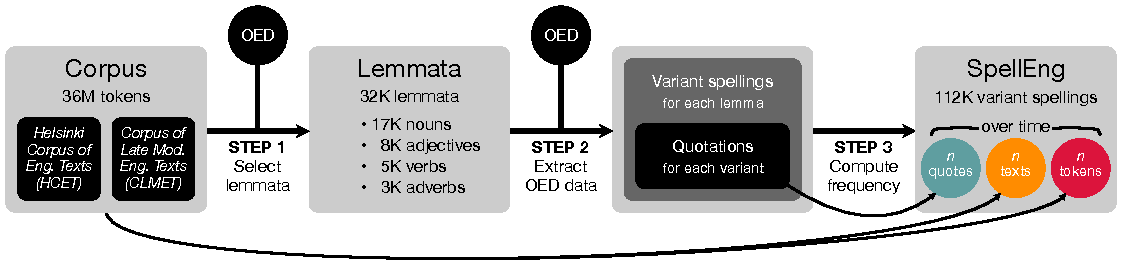
\includegraphics[]{figs/pipeline.pdf}}
	\vspace*{2pt}
	\caption{Overview of the construction of the SpellEng dataset. We first select the lemmata based on the words present in the historical corpus. We then access the OED entry for each lemma and extract the variant forms and usage quotations. Finally, we count how often each variant is used over time, both in the OED and in the corpus.}
	\label{pipeline}
	\end{figure}

The second step was to access the corresponding OED entry for each lemma and extract (a) all non-inflected variant spellings with their usage periods and (b) all usage quotations with their citation years. We then associated each usage quotation with the variant spelling that it made use of. The result is that each lemma is mapped to one or more variant spellings (minimally, the headword form itself is a variant spelling), and each variant spelling is mapped to zero or more quotations (some variants listed in the OED are not supported by quotational evidence).

The final step was to compute the frequencies of the variant spellings over time, which we do in two distinct ways. The first is to count the number of OED quotations associated with a given variant spelling. This is highly reliable because each quotation is a genuine example of a given lemma that has been verified by the OED's lexicographers. However, in some cases the number of quotations in an OED entry is relatively small, and it is also possible that the quotations may represent a skewed sample because they have been actively chosen rather than randomly sampled. We therefore also count the number of occurrences of each variant in the historical corpus, albeit with the possibility for mapping errors, since there is no automated way to verify that a given token in the corpus is indeed a genuine use of a particular lemma. We show later that these two methods tend to produce similar results.

Strictly, we define a variant spelling as an orthographic rendering of the pronunciation of the headword form (in the pronunciation of the time of the variant). For example, the lemma \lemma{lord}{n} has 29 variant spellings (\spelling{hlabard}, \spelling{hlafard}, \spelling{hlafor}, \spelling{hlaford}, \spelling{hlauerd}, \spelling{laferd}, \spelling{laferrd}, \spelling{laford}, \spelling{laird}, \spelling{lard}, \spelling{larde}, \spelling{lauer}, \spelling{lauerd}, \spelling{lauerde}, \spelling{leard}, \spelling{lhoauerd}, \spelling{lhord}, \spelling{lhorde}, \spelling{loard}, \spelling{loord}, \spelling{loorde}, \spelling{lor}, \spelling{lord}, \spelling{lorde}, \spelling{louerd}, \spelling{louerde}, \spelling{lourd}, \spelling{loverd}, \spelling{lowerd}), but not all of these are necessarily graphic renderings of the modern pronunciation \pronunciation{lɔrd}, since the word has gradually changed in pronunciation over time. To a certain extent, then, the SpellEng dataset unavoidably captures changes in pronunciation over time, and not changes that are purely graphic in nature. Likewise, it is difficult to avoid the fact that some spelling variants are motivated by different pronunciations across contemporaneous dialects (e.g., the Scottish form \spelling{laird} above, which is presumably spelled in a distinct way due to a distinct pronunciation). Our methodology does, however, avoid including inflected forms as variants (e.g., the plural form \spelling{lorddes} or the genitive form \spelling{lordene}).

\subsection{Preparation of the corpus}

We began by assembling a historical corpus of English by combining the \textit{Helsinki Corpus of English Texts} (HCET),\footnote{Version 0.96 of the TEI XML Edition downloaded from \url{https://helsinkicorpus.arts.gla.ac.uk}.} which covers the Old, Middle, and Early Modern periods of English, with the \textit{Corpus of Late Modern English Texts} (CLMET),\footnote{Version 3.1 downloaded from \url{https://fedora.clarin-d.uni-saarland.de/clmet/clmet.html}.} which covers the Late Modern period. Each of the corpora is divided into bands spanning between 70 and 100 years, and CLMET picks up where HCET leaves off in 1710. We merged the Old English~I and~II sections of HCET because Old English~I contained very little data (around 2000 word tokens across 10 texts) and because the resulting merger more closely aligned with the OED's classification of Old English into three, rather than four, periods (which will become relevant shortly). We performed several preprocessing steps on the raw corpus data. This included reducing everything to lowercase, removing all punctuation, and removing any tokens that did not consist purely of alphabetical characters (the standard 26 letters of the modern English alphabet plus \spelling{æ ð þ ę ł ȝ}). We also stripped anything from HCET that was tagged as marginalia or foreign language material. After applying these transformations, the overall corpus included 36 million tokens (313,234 types) across 762 texts. Table~\ref{banding} provides a breakdown of the size of the combined corpus by band.\footnote{Note that our word counts are slightly lower than the counts reported in the original corpora, since we have a more restrictive definition of a token that excludes e.g., numbers and foreign language material.}

	\begin{table}
	\begin{center}
	\begin{threeparttable}
	\caption{Historical banding and corpus count statistics}
	\footnotesize
	\begin{tabular}{llllrrrr}
	\toprule
	Band & Period & Corpus & Corpus section & $N$ years & $N$ texts & $N$ tokens & $N$ types \\
	\midrule
	 1 & Pre-950    & HCET  & Old English I \& II      & >100 &  31 & 88,820     & 15,327 \\
	 2 & 950--1049  & HCET  & Old English III          &  100 &  91 & 243,538    & 36,060 \\
	 3 & 1050--1149 & HCET  & Old English IV           &  100 &  28 & 64,063     & 11,179 \\
	 4 & 1150--1249 & HCET  & Middle English I         &  100 &  31 & 108,065    & 16,813 \\
	 5 & 1250--1349 & HCET  & Middle English II        &  100 &  22 & 95,183     & 12,561 \\
	 6 & 1350--1419 & HCET  & Middle English III       &   70 &  45 & 181,737    & 19,078 \\
	 7 & 1420--1499 & HCET  & Middle English IV        &   80 &  46 & 210,988    & 23,622 \\
	 8 & 1500--1569 & HCET  & Early Modern English I   &   70 &  44 & 188,709    & 19,267 \\
	 9 & 1570--1639 & HCET  & Early Modern English II  &   70 &  48 & 186,920    & 16,989 \\
	10 & 1640--1709 & HCET  & Early Modern English III &   70 &  46 & 169,225    & 13,466 \\
	11 & 1710--1779 & CLMET & Late Modern English I    &   70 &  88 & 10,351,523 & 90,928 \\
	12 & 1780--1849 & CLMET & Late Modern English II   &   70 &  99 & 11,190,347 & 108,347 \\
	13 & 1850--1919 & CLMET & Late Modern English III  &   70 & 143 & 12,440,365 & 116,911 \\
	\bottomrule
	\end{tabular}
	\label{banding}
	\end{threeparttable}
	\end{center}
	\end{table}

\subsection{Selection of the lemmata}

The next stage was to select a set of lemmata for which we could study spelling variation over time. To make this selection, we first isolated all unique wordforms of at least three characters that occurred in at least two texts within the same band. Additionally, for the Late Modern section, we only selected tokens tagged as NN (noun), JJ (adjective), VB (verb), or RB (adverb), which has the effect of filtering out inflected forms, since these are given other tags (e.g., NNS for plural nouns). This resulted in 64,139 unique wordforms. To map each wordform to a lemma, the wordform was searched in the OED, yielding a list of search results (OED entries) which was initially cached. We then mapped each corpus token to a lemma (i.e., an OED entry) by taking the first OED entry in the cached search results list that was (a) consistent with the text's year and (b), in the case of Late Modern, consistent with the token's part of speech tag.

We then selected all noun, adjective, verb, and adverb lemmata that were found to occur at least twice anywhere in the corpus. Additionally, we filtered out any lemma whose headword form appears on a list of 130 stop words (e.g., \textit{just}, \textit{have}, \textit{may}) and cases where the lemma's headword form contains capital letters (e.g., \textit{Trojan}, \textit{ABC}), punctuation (e.g., \textit{inst.}), or accented characters (e.g., \textit{naïveté}), indicating that the lemma is a proper noun, abbreviation, or loan word that has not been fully nativized. This resulted in 32,264 lemmata (16,932 nouns, 7,743 adjectives, 4,967 verbs, and 2,622 adverbs).

The lemmata are intended to represent a wide array of meanings from across the history of the English language, although there is likely to be a bias towards more modern lemmata given the larger size of the later sections of the corpus and the accuracy with which the OED's search tool is able to correctly recognize older wordforms. The most frequent noun lemmata were: \lemma{man}{n}, \lemma{time}{n}, \lemma{day}{n}, \lemma{thing}{n}, \lemma{sir}{n}, \lemma{life}{n}, \lemma{hand}{n}, \lemma{lady}{n}, \lemma{way}{n}, and \lemma{lord}{n}. The most frequent adjectives were: \lemma{good}{adj}, \lemma{great}{adj}, \lemma{least}{adj}, \lemma{little}{adj}, \lemma{first}{adj}, \lemma{many}{adj}, \lemma{old}{adj}, \lemma{young}{adj}, \lemma{much}{adj}, and \lemma{new}{adj}. The most frequent verbs were: \lemma{say}{v}, \lemma{make}{v}, \lemma{see}{v}, \lemma{come}{v}, \lemma{know}{v}, \lemma{take}{v}, \lemma{think}{v}, \lemma{give}{v}, \lemma{go}{v}, and \lemma{find}{v}. The most frequent adverbs were: \lemma{well}{adv}, \lemma{never}{adv}, \lemma{yet}{adv}, \lemma{even}{adv}, \lemma{ever}{adv}, \lemma{still}{adv}, \lemma{soon}{adv}, \lemma{however}{adv}, \lemma{far}{adv}, and \lemma{always}{adv}. At the other end of the frequency distribution, lemmata with just two occurrences in the corpus include nouns such as \lemma{dipsomania}{n}, \lemma{mudbank}{n}, and \lemma{sternutation}{n}, adjectives such as \lemma{heteroclite}{adj}, \lemma{parabolical}{adj}, and \lemma{snobby}{adj}, verbs such as \lemma{buttress}{v}, \lemma{disillusion}{v}, and \lemma{tattle}{v}, and adverbs such as \lemma{docilely}{adv}, \lemma{quizzically}{adv}, and \lemma{skittishly}{adv}.

\subsection{Extraction of the OED data}

For each lemma, we accessed the corresponding OED entry and parsed its ``Variant Forms'' section, which lists variant forms of the lemma along with their time periods of attested usage \parencite[see][for discussion]{Durkin:2016}. Additionally, if a given variant is dialectal, inflectional, or a possible error, it will usually be labeled as such. The OED is currently undergoing a long-term modernization effort and, at the time of parsing, around half of the Variant Forms sections we extracted had been updated to a machine-readable tabular format (e.g., \lemma{interest}{n}), while the other half were textual descriptions that had to be parsed. For example, the Variant Forms section for \lemma{trick}{n} reads:
\begin{quote}
Middle English--1500s \textbf{trik}, plural \textbf{trikkes}, 1500s--1600s \textbf{tricke}, 1500s-- \textbf{trick}, (1600s \textbf{trike}).
\end{quote}
From this description, we must ignore the plural form \spelling{trikkes} and extract the four non-inflected variants and their usage periods: \spelling{trik} (1150--1599), \spelling{tricke} (1500--1699), \spelling{trick} (1500--2099), and \spelling{trike} (1600--1699).
Parsing these descriptions is not always straightforward, however, since they are often written in inconsistent or ambiguous ways. For example, sometimes inflection labels are placed before the variant (e.g., ``plural trikkes''). In other cases, the labels are placed in parentheses after the variant (e.g., for \lemma{bank}{n}: ``bonkkes (plural)'') or a single label might apply to multiple variants (e.g., for \lemma{echo}{n}: ``Plural echoes, rarely echos''). In addition, sometimes the OED lists variants in an abbreviated way; for \lemma{serenity}{n}, the OED lists \mbox{``-yte''} and \mbox{``-itie''} as possible variants, which must be expanded into \spelling{serenyte} and \spelling{serenitie}. Likewise, for \lemma{step}{n}, the OED lists ``stepp(e'' as a variant, which must be expanded into \spelling{stepp} and \spelling{steppe}. In cases where the Variant Forms section cross-references derivational affixes, we follow the cross-references and derive all possible spellings. For example, for \lemma{painful}{adj}, whose Variant Forms section reads, ``See \textit{pain n.1} and \textit{-ful suffix},'' we derive possible spellings such as \spelling{payenfulle}, \spelling{paynfull}, and \spelling{peynful} by concatenating the variant spellings listed in the cross-referenced entries.

Our script extracts as many of the variant forms as possible, while attempting to ignore anything labeled as an inflection or error.\footnote{Specifically, we ignore anything with the following labels: 2nd, 3rd, abbreviation, accusative, adverb, chiefly in sense, comparative, dative, error, genitive, imperative, infinitive, inflected, participle, past, plural, sic, subjunctive, superlative.} In this way, we aim to isolate the nominative singular in the case of nouns, the present-tense base form in the case of verbs, and the positive form in the case of adjectives, although it is not always possible to isolate these forms perfectly, especially in the case of common verbs where the OED supplies rich information about the verbal inflections present in Old and Middle English. We do not attempt to exclude variants labeled as belonging to a particular dialect (e.g., ``Anglo-Irish,'' ``Mercian,'' ``York,'' etc.), since there is no principled way to define which dialect(s) of English should be included or excluded. As a result, our dataset does not perfectly isolate spelling variation (i.e., variation that is purely graphic in nature), since, to some extent, the spelling variants we identify may be motivated by differences in pronunciation across dialects.

	\begin{table}
	\begin{center}
	\begin{threeparttable}
	\caption{Variant spellings and quotations extracted for \lemma{disloyalty}{n}}
	\footnotesize
	\begin{tabular}{ll p{10.5cm}}
	\toprule
	Variant & Citation year & Quotation \\
	\midrule
	\spelling{disloyalte}  & 1481 (Band~7) & Whan the \textbf{disloyalte} and falsenes of mahomet ran thurgh thoryent. \\
	\spelling{desloyalte}  & 1484 (Band~7) & He slewe his broder Amon that suche \textbf{desloyalte} and vntrouth had done to his suster. \\
	\spelling{disloyaltie} & 1600 (Band~9) & Some ... charged him with \textbf{disloyaltie}, saying that he would not fight, having beene corrupted. \\
	                       & 1600 (Band~9) & There shal appeere such seeming truth of Heroes \textbf{disloyaltie}, that iealousie shal be cald assurance. \\
	\spelling{disloyalty}  & 1647 (Band~10) & Although Richard the first forgot this mans \textbf{disloyalty}, yet God remembred it. \\
	                       & 1712 (Band~11) & This Princess was then under Prosecution for \textbf{Disloyalty} to the King's Bed. \\
	                       & 1821 (Band~12) & Discontent and \textbf{disloyalty}, like the teeth of the dragon, He had sown on the winds. \\
	                       & 1846 (Band~12) & Several of the Sipahis ... suffered the penalty of their \textbf{disloyalty}. \\
	                       & 1874 (Band~13) & The infidelity to truth, the \textbf{disloyalty} to one's own intelligence. \\
	\bottomrule
	\end{tabular}
	\label{extraction_example}
	\end{threeparttable}
	\end{center}
	\end{table}

We also extracted the usage quotations from each OED entry, which provide examples of the lemma being used in sentence contexts that are dated to specific years or time periods (see Table~\ref{extraction_example} for an example). We extracted all quotations where the spelling of the target word within the quotation was one of the variants identified previously. Thus, if the quotation used an inflected form, it would be ignored. In addition, we only accepted a quotation if its citation year fell within the variant's usage period in order to avoid mapping inflected forms from one period to non-inflected variants from another. For example, for \lemma{horn}{n}, the OED lists \spelling{horne} as a possible variant spelling in Middle English, but among the quotations we find ``Singað in fruman monðes horne'' dated to Old English. However, ``horne'' here is in~fact the Old English dative case, and so should not be counted as an instance of the variant spelling \spelling{horne}. In other words, in Old English, there's a meaningful and phonetic difference between the words \textit{horn} and \textit{horne}, while in Middle English the two are merely variant spellings of the same word, which is what our dataset aims to capture.

Each extracted quotation was mapped to its corresponding historical band based on the citation year. In the case of quotations from Old English, the OED usually gives the citation year as ``eOE'', ``OE'', or ``lOE'', which we map respectively to Bands~1, 2, and~3.\footnote{This results in a slight discrepancy with the HCET banding, since the OED adopts 1100 as the boundary between Old English and Late Old English, where HCET adopts 1050. https://www.oed.com/discover/old-english-in-the-oed} In the case of Middle and Early Modern English, the citation years are often prepended with ``c'' (circa) or ``a'' (ante). We treat circa years as if they were definite and map the quotations to the corresponding bands accordingly. In the case of ante years, we subtract 10 to push the quotation into an earlier band if its year falls close to a band boundary (e.g., ``a1500'' will be mapped to Band~7 rather than Band~8). For Middle English quotations, it is common for two citation years to be provided: a manuscript year (the year when the source manuscript is believed to have been produced) and a composition year (an earlier year when the original work is believed to have been written).\footnote{https://www.oed.com/discover/dating-middle-english-evidence-in-the-oed} In these cases, we adopt the manuscript year, since our aim is to track which variants were actually being \textit{written} at a given point in time, regardless of whether those variants were contemporary spellings or preserved spellings.

\subsection{Calculating the frequency of spelling variants}

	\begin{table}
	\begin{center}
	\begin{threeparttable}
	\caption{Frequency of spelling variants of \lemma{king}{n} by historical band (OED quotation count)}
	\footnotesize
	\begin{tabular}{lrrrrrrrrrrrrr}
	\toprule
	Variant & 1 & 2 & 3 & 4 & 5 & 6 & 7 & 8 & 9 & 10 & 11 & 12 & 13 \\
	\midrule
	\spelling{cing}   & - & 1 & - & - & - & - &  - & - &  - &  - &  - &  - &  - \\
	\spelling{cyng}   & - & 1 & 2 & - & - & - &  - & - &  - &  - &  - &  - &  - \\
	\spelling{cyning} & 4 & 4 & 1 & - & - & - &  - & - &  - &  - &  - &  - &  - \\
	\spelling{king}   & - & - & 1 & 3 & 4 & 4 &  4 & 6 & 37 & 45 & 38 & 65 & 73 \\
	\spelling{kinge}  & - & - & - & - & 3 & - &  2 & 1 &  - &  - &  - &  - &  - \\
	\spelling{kyng}   & - & - & 1 & 2 & 3 & 8 & 10 & 8 &  1 &  - &  - &  - &  - \\
	\spelling{kynge}  & - & - & - & - & 1 & 1 &  4 & 5 &  - &  - &  - &  - &  - \\
	\spelling{kyning} & - & 1 & - & - & - & - &  - & - &  - &  - &  - &  - &  - \\
	\bottomrule
	\end{tabular}
	\label{king_oed_count}
	\end{threeparttable}
	\end{center}
	\end{table}

The set of quotations extracted from a given OED entry acts as a kind of micro-corpus, allowing us to calculate how often each attested variant spelling was being used in each historical band. An example for \lemma{king}{n} is shown in Table~\ref{king_oed_count}. In Band~1, the only attested spelling is \spelling{cyning}. The modern spelling \spelling{king} first enters in Band~3, ultimately becoming dominant in Band~9, although it was also eclipsed by the spelling \spelling{kyng} for a few centuries. These frequency estimates derived from the OED quotations have the benefit of being based on genuine uses of a particular lemma that have been painstakingly collated and verified by the OED's lexicographers. However, there are also a number of limitations to relying solely on the OED quotation counts. Firstly, in the case of lower-frequency words, there tend to be few quotations and often no examples at all for some spellings. This results in more uncertainty about the true proportion with which different spellings were being used in a given band; it also frequently results in ties regarding which spelling was dominant in a given period. Secondly, the set of OED quotations may represent a biased sample that favors certain spellings over others. For example, there may be a tendency to favor certain types of source over others (e.g., books over letters), or there may be a preference for standard spellings over non-standard ones. Indeed, it is also possible that rare variant spellings might be over-represented, since some quotations may have been selected precisely because they provide an example of a low-frequency spelling.

We therefore turn back to the historical corpus to verify and supplement the frequency estimates derived from the OED quotations. As with the OED counts, we only count an occurrence of a variant spelling in the corpus if it falls within the variant's usage period (as extracted from the Variant Forms section of the OED entry) to avoid mapping variants from one period to inflected forms or other lemmata from another period. For example, the spelling \spelling{kink} for \lemma{king}{n}, whose usage period is given as 1150--1699, is correctly ignored in the post-1700 corpus sections where it is used for a different lemma (\lemma{kink}{n}). In the case of the Late Modern bands, we also match for word class, which further reduces the chance of attributing an occurrence of a variant to the wrong lemma or an inflected form.

We use the corpus to produce two distinct counts: the number of tokens of a given variant spelling (for each historical band) and the number of texts in which a given variant occurs (for each historical band). These two counts reflect slightly different assumptions. The token count is a direct measure of how many times a given spelling occurred in the corpus; however, it may give a biased impression of how likely it was for a given spelling to be selected by a writer, since it treats tokens as independent. In reality, the instances of a given spelling within a text are unlikely to be independent from each other, since a given text will typically be written by a single author, transcribed by a single scribe, or edited by a single copy~editor applying a house~style, potentially leading to biased estimates of the relative popularity of different spellings. For example, imagine a scenario in which a given band contains ten texts, one of which uses the spelling \spelling{kyng} 100 times, while the other nine texts each use the spelling \spelling{king} once. The token count will give the impression that \spelling{kyng} is more common than \spelling{king} (100 tokens vs.\@ 9 tokens), whereas the text count will give the impression that \spelling{king} is more common than \spelling{kyng} (9 texts vs.\@ 1 text). The text count therefore reflects something closer to the number of times a spelling was independently chosen by a writer, whereas the token count reflects something closer to the number of times a reader might encounter a spelling, after accounting for general word frequency.

	\begin{table}
	\begin{center}
	\begin{threeparttable}
	\caption{Frequency of spelling variants of \lemma{king}{n} by historical band (corpus text count)}
	\footnotesize
	\begin{tabular}{lrrrrrrrrrrrrr}
	\toprule
	Variant & 1 & 2 & 3 & 4 & 5 & 6 & 7 & 8 & 9 & 10 & 11 & 12 & 13 \\
	\midrule
	\spelling{cinc} & - & 1 & - & - & - & - & - & - & - & - & - & - & - \\
	\spelling{cincg} & - & 2 & - & - & - & - & - & - & - & - & - & - & - \\
	\spelling{cing} & 2 & 3 & 5 & - & - & - & - & - & - & - & - & - & - \\
	\spelling{cingc} & - & 1 & - & - & - & - & - & - & - & - & - & - & - \\
	\spelling{cininc} & - & - & 1 & - & - & - & - & - & - & - & - & - & - \\
	\spelling{cining} & - & 7 & 2 & - & - & - & - & - & - & - & - & - & - \\
	\spelling{ciningc} & - & 1 & - & - & - & - & - & - & - & - & - & - & - \\
	\spelling{cync} & - & 1 & - & - & - & - & - & - & - & - & - & - & - \\
	\spelling{cyncg} & - & 1 & - & - & - & - & - & - & - & - & - & - & - \\
	\spelling{cyng} & 1 & 7 & 6 & 2 & - & - & - & - & - & - & - & - & - \\
	\spelling{cyngc} & - & 1 & 1 & - & - & - & - & - & - & - & - & - & - \\
	\spelling{cynig} & - & 2 & - & - & - & - & - & - & - & - & - & - & - \\
	\spelling{cynin} & 1 & - & - & - & - & - & - & - & - & - & - & - & - \\
	\spelling{cyninc} & - & 1 & - & - & - & - & - & - & - & - & - & - & - \\
	\spelling{cynincg} & - & 4 & - & - & - & - & - & - & - & - & - & - & - \\
	\spelling{cyning} & 10 & 30 & 6 & - & - & - & - & - & - & - & - & - & - \\
	\spelling{cyningc} & - & 5 & 1 & - & - & - & - & - & - & - & - & - & - \\
	\spelling{cynng} & 1 & - & - & - & - & - & - & - & - & - & - & - & - \\
	\spelling{kin} & - & - & - & 2 & 1 & - & - & - & - & - & - & - & - \\
	\spelling{king} & - & 2 & - & 15 & 11 & 10 & 5 & 16 & 17 & 20 & 57 & 72 & 92 \\
	\spelling{kinge} & - & - & - & 11 & 3 & - & 2 & 8 & 8 & 2 & - & - & - \\
	\spelling{kingue} & - & - & - & - & 1 & - & - & - & - & - & - & - & - \\
	\spelling{kining} & - & 1 & 2 & - & - & - & - & - & - & - & - & - & - \\
	\spelling{kink} & - & - & - & - & 1 & - & - & - & - & - & - & - & - \\
	\spelling{kyncg} & - & 1 & - & - & - & - & - & - & - & - & - & - & - \\
	\spelling{kyng} & - & - & 2 & 4 & 9 & 21 & 27 & 11 & 1 & - & - & - & - \\
	\spelling{kynge} & - & - & - & 1 & 5 & 2 & 21 & 11 & - & - & - & - & - \\
	\spelling{kyning} & 4 & 4 & 2 & 1 & - & - & - & - & - & - & - & - & - \\
	\spelling{kyningc} & 1 & - & - & - & - & - & - & - & - & - & - & - & - \\
	\bottomrule
	\end{tabular}
	\label{king_corpus_count}
	\end{threeparttable}
	\end{center}
	\end{table}

Table~\ref{king_corpus_count} provides the corpus text counts for \lemma{king}{n}. Although there is generally a high level of agreement with the OED quotation counts (Table~\ref{king_oed_count}), the corpus provides richer evidence for this particular lemma, especially with regards to the lower frequency variants (e.g., \spelling{cync}, \spelling{kin}, and \spelling{kingue}) for which the OED provides no example quotations at all.\footnote{However, this is not always the case. For \lemma{abandon}{v}, for example, the only variant present in the corpus is the modern spelling \spelling{abandon}, while the OED provides example quotations for nine additional spellings: \spelling{abandone}, \spelling{abandoun}, \spelling{abandoune}, \spelling{abandune}, \spelling{abawndone}, \spelling{habandone}, \spelling{habandoune}, \spelling{habondone}, and \spelling{habounden}.} In terms of the dominant form in each band, both sources agree on all but Band~8, where the OED says \spelling{kyng} (8 quotations) is more frequent than \spelling{king} (6 quotations), while the corpus says \spelling{king} (16 texts) is more frequent than \spelling{kyng} (11 texts). Nevertheless, the two sources do agree that the only four spellings in~use in Band~8 were \spelling{king}, \spelling{kinge}, \spelling{kyng}, and \spelling{kynge}.

Although the corpus counts (both the text count and the token count) generally tend to provide richer evidence, they are also likely to be somewhat unreliable because only the Late Modern section of the corpus is part-of-speech tagged and none of the corpus is lemma-tagged. As a consequence, it is impossible to determine automatically whether an instance of a particular spelling in the corpus is in~fact a genuine use of a particular lemma. For example, perhaps the two texts that use the spelling \spelling{cing} in Band~1 of the corpus are using that spelling for some entirely unrelated lemma. Therefore, our dataset provides all three variant counts---the OED quotation count, the corpus text count, and the corpus token count. The choice of which count to use will depend on one's research question and the tradeoffs one is willing to make. To summarize:
\begin{enumerate}
\item \textbf{The OED quotation count} is the number of quotations in the lemma's OED entry that use a given spelling within a given band. These counts are highly reliable because the quotations have been manually verified as genuine uses of a lemma by experienced lexicographers. However, the quotation count may be skewed in important ways, since the quotations have presumably been actively selected by the OED's lexicographers rather than randomly sampled.
\item \textbf{The corpus text count} is the number of texts that contain at least one occurrence of a given variant spelling within a given band. It is similar to the quotation count in the sense that it represents the number of times a given variant was independently chosen, but may be less biased than the quotation count to the extent that the corpus represents a random sample of English texts. Its main weakness is that the mere occurrence of a given spelling in a text is no guarantee that the occurrence is in fact a genuine use of the lemma.
\item \textbf{The corpus token count} is the total number of times a given spelling occurs in the corpus within a given band. It is therefore guaranteed to be greater than or equal to the text count. Like the text count, there is no guarantee that all occurrences of a given spelling are genuine uses of a particular lemma, but the advantage of the token count is that the numbers are typically one or two orders of magnitude larger than the text count or quotation counts, providing more nuanced evidence about the relative proportions with which a set of variants are used. The token count also factors in the general frequency of the lemma and is therefore a better estimate of how likely it is that a spelling would be encountered by a reader.
\end{enumerate}

\subsection{Structure of the dataset}

The SpellEng dataset, as well as the Python code used to create it, is freely available from the OSF repository associated with this project (\url{https://osf.io/jtb4m/}) or from GitHub (\url{https://github.com/jwcarr/spelleng}). It is provided in the form of three CSV files: \texttt{spelleng\_v1\_quote.csv}, \texttt{spelleng\_v1\_text.csv}, and \texttt{spelleng\_v1\_token.csv}. Each file contains the relevant counts for 112,080 variant spellings (column \texttt{variant}) across the 32,264 lemmata (column \texttt{lemma\_id}). The dataset does not necessarily include all variants reported in the OED; only those variants that were attested at least once in either the quotations or corpus are included. SpellEng provides counts for each of the 13 historical bands (columns \texttt{band1} through \texttt{band13}), as listed in Table~\ref{banding}, and the counts are also broken down into the four major periods of the history of English (columns \texttt{oe}, \texttt{me}, \texttt{eme}, \texttt{lme}), permitting analysis with higher time resolution (but smaller sample sizes) or lower time resolution (but larger sample sizes). We use the same lemma IDs as the OED to aid cross-referencing (e.g., \texttt{banshee\_n} corresponds to the OED entry at \url{https://www.oed.com/dictionary/banshee_n}). The \texttt{headword} and \texttt{pos} columns provide the OED headword form separately from the part of speech tag, which is given in the conventional corpus-analysis format (\texttt{nn}, \texttt{vb}, \texttt{jj}, \texttt{rb}). Note that headword forms are not unique to lemmata, since there are frequently lemmata that share a headword form (e.g., \lemma{wind}{n} and \lemma{wind}{v}).

\subsection{Validation of the dataset}

Extracting the variant forms from the OED is complex and error prone, not only because the Variant Forms sections are often written inconsistently, but also because language itself is messy and complex. To validate the dataset, we performed a random spot check of 150 lemmata (around 0.5\% of the dataset). In general, we found that the extraction of the variant forms and the mapping of the quotations to those forms by historical band was very reliable. However, the removal of inflected forms was not always perfect, especially in the case of high frequency verbs where it can be particularly difficult to separate spelling variation from inflection. In the case of \lemma{see}{v}, for example, SpellEng lists \spelling{sees} as a variant spelling. The reason for this is that the word \textit{sees} is a possible rendering of the first person singular in some dialects (e.g., ``I sees him now and again'') and is therefore listed as a variant in the OED. Consequently, the form \spelling{sees} finds itself in the SpellEng dataset. Importantly, the spelling \spelling{sees} will be highly confounded with third person uses, leading to the overestimation of its frequency, although in this particular case, no occurrences are counted in the Late Modern section of the corpus thanks to the part-of-speech tagging, which uses a distinct tag for third person verbs.

To perform a more quantitative validation of the dataset, we take advantage of the fact that we have counts from two distinct sources (the OED quotations and the corpus). If the two sources tend to agree on which spelling was dominant in each band, we might have increased confidence in the dataset as a whole. For each band and each lemma, the two sources may be said to agree when one of two conditions is met:
\begin{enumerate}
\item If both sources have a count of zero for all variants, the two sources are in agreement; they agree that the lemma is unattested in that band.
\item If both sources count at least one variant, then the two sources are in agreement if they agree on which variant was most frequent in a given band.\footnote{To resolve ties, the dominant form(s) from one source must be a subset of the dominant form(s) in the other. For example, if one source says that \spelling{cyng} is dominant and the other source says that \spelling{cyng} and \spelling{cynging} are co-dominant, this still counts as agreement.}
\end{enumerate}
If neither condition is met, the sources are said to disagree. Thus, for each lemma, we can compute an agreement score that ranges between 0 and 13---the number of bands in which the two sources agree. The distribution of agreement scores is plotted in Fig.~\ref{agreement}. The majority of lemmata tend to have a high level of agreement (mean: 10.2; median: 11; mode: 11). When agreement is low (e.g., $< 8$), this tends to indicate that the lemma is confounded with other lemmata, which is especially common among short words. For example, \lemma{ear}{n} has a very low score of 1 because its variant spellings (e.g., \spelling{here}, \spelling{ire}, \spelling{year}) are highly confounded with other lemmata, which leads to spurious results when counting the corpus (and therefore poor agreement with the OED data). In cases such as these, the OED data should be preferred.

	\begin{figure}
	\makebox[\textwidth][c]{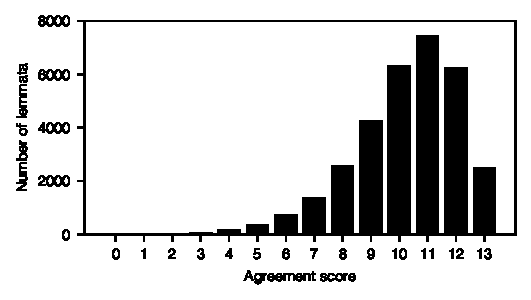
\includegraphics[]{figs/agreement.pdf}}
	\vspace*{2pt}
	\caption{Distribution of agreement scores. The agreement score is the number of bands in which the OED and corpus data agree on which variant spellings was dominant.}
	\label{agreement}
	\end{figure}

\subsection{General properties of the dataset}

	\begin{figure}
	\makebox[\textwidth][c]{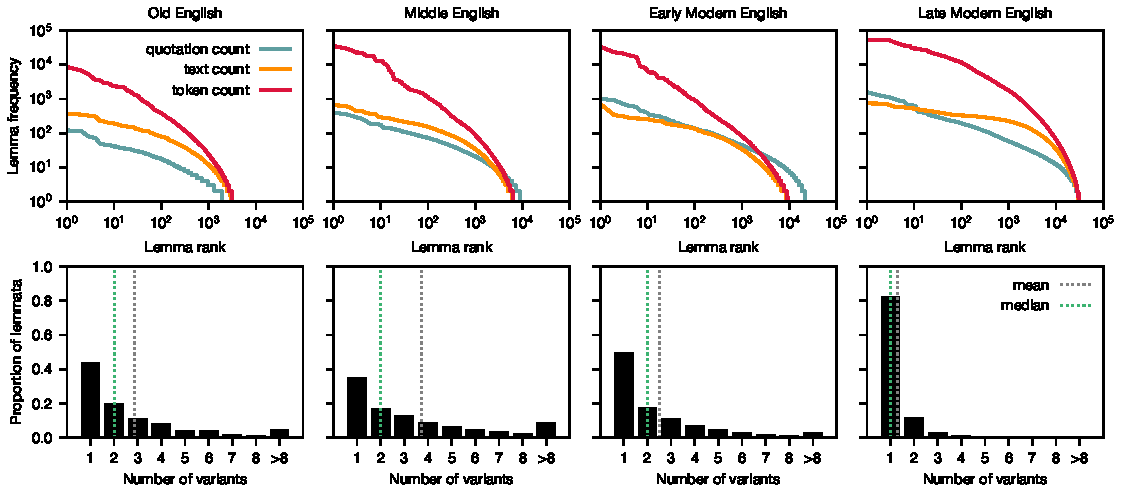
\includegraphics[]{figs/frequency_plot.pdf}}
	\vspace*{2pt}
	\caption{\textbf{\textsc{top}} Lemma frequency against lemma rank (on log--log axes) for each major period of English. The corpus counts are generally larger than the OED quotation counts, although in some cases, such as the lower ranking lemmata in Early Modern English, the OED quotation counts outperform the corpus. \textbf{\textsc{bottom}} Proportion of lemmata that have one through eight or more than eight variant spellings (attested in either the corpus or the OED entry). By the Late Modern period, some 80\% of lemmata have only one variant spelling.}
	\label{frequency_plot}
	\end{figure}

The top panels in Fig.~\ref{frequency_plot} show lemma frequency against lemma rank for each major period of English and for each of the three count methods. In the Old English period, the corpus text count tends to be around an order of magnitude larger than the quotation count, while in the later periods the two tend to be more closely aligned, which suggests that the corpus text count does not provide that much more information than the quotations. Indeed, in the Early Modern period (and to a lesser extent the Middle English period), the number of OED quotations for a lemma of given rank tends to be larger than the text count and sometimes even the token count (especially among lower ranking lemmata).

The bottom panels in Fig.~\ref{frequency_plot} give the proportion of lemmata that have one through eight (or more than eight) variant spellings that were attested in either the corpus or the OED entry. In the Late Modern period, there is little spelling variation, with some 80\% of lemmata having only one possible spelling. In the three earlier periods, the median number of variants per lemma is 2 and the distributions have longer tails indicating wider variation. By Band~13 (1850--1919), 93.7\% of lemmata had only one variant spelling, 5.2\% had two variants, and 1.1\% had three or more. Part of this remaining variation stems from the differences between the American and British standards (\spelling{analog}/\spelling{analogue}, \spelling{color}/\spelling{colour}, \spelling{generalize}/\spelling{generalise}, \spelling{theater}/\spelling{theatre}), but several other notable instances of variation remain, some of which have persisted to the present day. This includes:
\begin{itemize}
	\item the use of double letters: \spelling{gamon}/\spelling{gammon}, \spelling{pupilage}/\spelling{pupillage}, \spelling{rackety}/\spelling{racketty};
	\item the use of final-\spelling{e}: \spelling{proletariat}/\spelling{proletariate}, \spelling{volt}/\spelling{volte}, \spelling{whilom}/\spelling{whilome};
	\item the choice of vowel grapheme: \spelling{equatoreal}/\spelling{equatorial}, \spelling{gargoyle}/\spelling{gurgoyle}, \spelling{pleasance}/\spelling{pleasaunce};
	\item the dropping of \spelling{e} before an affix: \spelling{lacey}/\spelling{lacy}, \spelling{sizeable}/\spelling{sizable}, \spelling{storeage}/\spelling{storage};
	\item the transformation of \spelling{y} into \spelling{i} before an affix: \spelling{gayety}/\spelling{gaiety}, \spelling{honeyed}/\spelling{honied}, \spelling{slyly}/\spelling{slily};
	\item the choice of \spelling{c} vs.\@ \spelling{k}: \spelling{disc}/\spelling{disk}, \spelling{embarcation}/\spelling{embarkation}, \spelling{mimic}/\spelling{mimik};
	\item the representation of palatalization before \spelling{i}: \spelling{connection}/\spelling{connexion}, \spelling{spacially}/\spelling{spatially}, \spelling{vicious}/\spelling{vitious};
	\item the simplification of the \spelling{ae} digraph: \spelling{aether}/\spelling{ether}, \spelling{laesion}/\spelling{lesion}, \spelling{sphæroid}/\spelling{spheroid};
	\item and other idiosyncrasies: \spelling{dumby}/\spelling{dummy}, \spelling{laggard}/\spelling{laggart}, \spelling{nickel}/\spelling{nickle}.
\end{itemize}

Although the number of variants per lemma gives us an indication of how much variation there is, it does not take into account the proportions with which those variants were used. Even if a word has many attested variants, it might still be the case that only one of them was in regular use, such that, in practice, the amount of variation that one can expect to experience is still quite low. A more formal measure of variation should take this into account, with variation being at its maximum when there are not just many variants, but many variants with equal frequency. This corresponds to the Shannon entropy, which is given by
\begin{equation}
H(V) = -\sum_{v \in V} \mathrm{Pr}(v) \log \mathrm{Pr}(v),
\end{equation}
where $V$ is a set of variants and $\mathrm{Pr}(v) = \mathrm{Freq}(v) / \sum_{v^\prime \in V} \mathrm{Freq}(v^\prime)$. 

Fig.~\ref{entropy_plot} plots variant entropy (averaging over lemmata) across the 13 historical bands and for each of the three count methods. The three methods generally paint the same picture, although the OED data tends to suggest a more gradual rise in variation over the Middle English period, where the corpus suggests a more sudden increase in Band~4. Overall, we find an inverse-\textsc{u} shaped curve: Relatively low levels of variation in Old English, followed by a period of high variation peaking in Band~7, and finally a gradual reduction in variation over the Early Modern period and near-fixity by Band~11. \textcite{Kupkova:2023} presents similar results in terms of variant entropy for the Early Modern period specifically. We now turn to the question of how, in the absence of a strong guiding hand, this process of standardization unfolded.

	\begin{figure}
	\makebox[\textwidth][c]{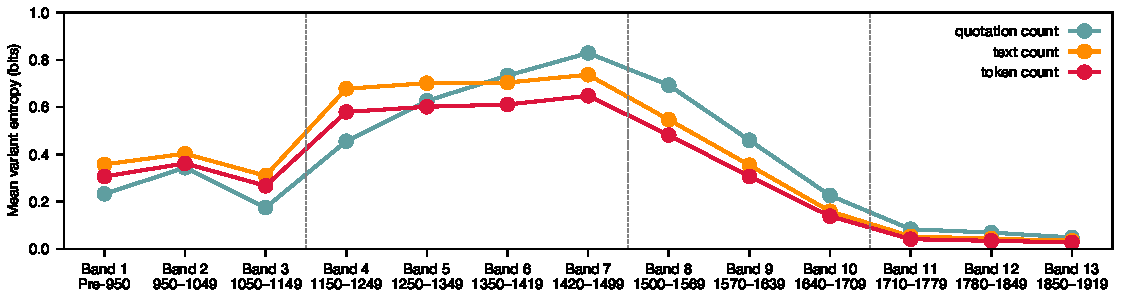
\includegraphics[]{figs/entropy_plot.pdf}}
	\vspace*{2pt}
	\caption{Mean variant entropy by historical band (i.e., average amount of uncertainty in the spelling of each lemma over time). Dashed gray lines mark the boundaries between Old, Middle, Early Modern, and Late Modern English. Entropy peaks in Band~7 and approaches 0 by Band~13.}
	\label{entropy_plot}
	\end{figure}

%~%~%~%~%~%~%~%~%~%~%~%~%~%~%~%~%~%~%~%~%~%~%~%~%~%~%~%~%~%~%~%~%~%~%~%~%~%~%~%~%~%~%~%~%~%~%~%~%~%~%~%

\section{Frequency-dependent selection in the English spelling system}

As noted in the Introduction, one (partial) way to explain the standardization of English is through a process of positive frequency-dependent selection. If a writer wishes to maximize the chance of being correctly and easily understood, it will be advantageous to select spelling variants that are frequent and therefore likely to be known to a future reader. Such a process would predict that the spelling variants frequent at one point in time should be disproportionately amplified at a subsequent point in time. Fig.~\ref{fds} illustrates this process for the lemma \lemma{fire}{n}: The population of reader/writers at time $t$ observes instances of four spelling variants that were produced by the population at time $t-1$, and subsequently they will go~on to produce new instances of those spelling variants that a future population at time $t+1$ will observe. Our goal is to understand what kind of selective force best explains the transition from the frequency distribution at time $t$ to the frequency distribution at time $t+1$.

\subsection{Model}

	\begin{figure}
	\makebox[\textwidth][c]{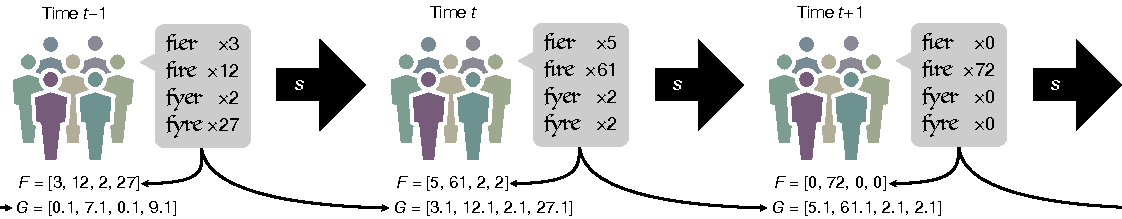
\includegraphics[]{figs/fds.pdf}}
	\vspace*{2pt}
	\caption{Model of frequency-dependent selection. The population of reader/writers at time $t$ observes the spelling variants produced by the population at time $t-1$ and produces spellings that will be observed at time $t+1$. At a given timepoint and for a given lemma, the model aims to establish what value of $s$ (the selection bias) would best explain frequency distribution $F$ given frequency distribution $G$. Example counts are given for the lemma \lemma{fire}{n} at Bands~8, 9, and~10.}
	\label{fds}
	\end{figure}

Our model shares various similarities with other cultural evolutionary models of frequency-dependent selection \parencite[e.g.,][]{Pagel:2019, Newberry:2022, GuerreroMontero:2023} and the more general class of iterated learning models \parencite[e.g.,][]{Griffiths:2007, KirbyDowmanGriffiths:2007, Reali:2009}. Our goal is to infer what selection bias $s$ would best explain an observed frequency distribution (over $m$ variants) for lemma $l$ and at timepoint $t$, denoted $F_{l,t}$, given the corresponding frequency distribution from the previous timepoint, denoted $G_{l,t}$ (as illustrated in Fig.~\ref{fds}). To do so, we adopt the following hierarchical Bayesian model:
\begin{align*}
            F_{l,t} & \sim \mathrm{DirMult}(n_{l,t}, \alpha_{l,t}) \\
       \alpha_{l,t} & = \frac{G_{l,t}^{1 + s_{l,t}} \cdot \sum G_{l,t}}{\sum G_{l,t}^{1 + s_{l,t}}} \\
            s_{l,t} & \sim \mathrm{Normal}(\mu_t, \sigma_t) \\
              \mu_t & \sim \mathrm{Normal}(\beta, \zeta) \\
           \sigma_t & \sim \mathrm{Gamma}(\gamma, \xi) \\
              \beta & \sim \mathrm{Normal}(0, 2) \\
              \zeta & \sim \mathrm{Exponential}(1) \\
             \gamma & \sim \mathrm{Gamma}(2, 0.5) \\
                \xi & \sim \mathrm{Exponential}(1)
\end{align*}
In brief, the model states that $F_{l,t}$ is related to $G_{l,t}$ through a latent parameter $s_{l,t}$ that represents the selection bias (which is what we aim to infer from the data). More specifically, the model assumes that frequency distribution $F_{l,t}$ is drawn from a Dirichlet-Multinomial distribution parameterized by a sample size, $n_{l,t} = \sum F_{l,t} = \sum_{i=1}^m f_{l,t,i}$, and a vector of concentration weights, $\alpha_{l,t}$, which is given by redistributing the counts from the previous timepoint according to the selection bias.\footnote{The Dirichlet-Multinomial distribution generalizes the Beta-Binomial distribution to more than two categorical outcomes (in our case, more than two possible variants). The Multinomial distribution tells us the likelihood of observing frequency distribution $F$ given sample size $n$ and probability distribution $p$. This probability distribution is linked to the previous frequency distribution $G$ through a Dirichlet prior that accounts for uncertainty in the previous counts. Since the Dirichlet distribution is parameterized by a vector of concentration weights, $\alpha$, that must be greater than zero, we apply additive smoothing to $G$ by adding $0.1$ to each count. Thus, variants with a count of zero at $t-1$ are assigned a small amount of probability mass, since the model would otherwise be unable to explain the innovation of new variant forms.} This selection bias, which is estimated for each lemma and at each timepoint, is assumed to come from a normal distribution, with each timepoint having its own distribution (with mean $\mu_t$ and standard deviation $\sigma_t$). These timepoint-specific means and standard deviations are themselves given hyperpriors ($\beta$, $\zeta$, $\gamma$, $\xi$), which encode a high-level, a-priori expectation that the selection bias will be approximately distributed around 0 with a standard deviation around 2.

Crucially, the $s$ parameter can be interpreted as follows:
\begin{itemize}
	\item $s = 0$: Neutral selection. The spelling variants at time $t$ are used in direct proportion to their counts at $t-1$. For example, a set of two variants with an 80\%--20\% distribution at time $t-1$ would continue to have an 80\%--20\% distribution at time $t$. Conceptually, this represents a situation in which spelling variation is stable over time; the relative popularity of variants remains consistent without any reinforcing or diversifying trends. This could occur, for example, if there is stable variation, such as the continued persistence of American and British variants that remain in roughly the same proportion over time.
	\item $s > 0$: Positive selection. Variants that were more frequent at $t-1$ are becoming even more frequent at time $t$, and variants that were less frequent at $t-1$ are becoming even less frequent. For example, an 80\%--20\% distribution might become 90\%--10\%, or a 40\%--30\%--20\%--10\% distribution might become 64\%--27\%--8\%--1\%. Conceptually, this represents a situation in which the distribution over variants becomes amplified or accentuated, with frequently used variants increasing in usage relative to less frequently used variants. Positive selection is therefore consistent with standardization.
	\item $s < 0$: Negative selection. Variants that were more frequent at time $t-1$ are becoming less frequent at time $t$, and variants that were less frequent at time $t-1$ are becoming more frequent. For example, two variant spellings with an 80\%--20\% distribution at time $t-1$ might become 70\%--30\% at time $t$, or four variants with a 40\%--30\%--20\%--10\% distribution might invert to become 10\%--20\%--30\%--40\%. Conceptually, this represents a situation of rapid change in variant usage, where less common forms are being adopted and used more frequently, potentially due to systematic changes to the spelling system as a whole, language contact, the introduction of entirely new variants, or the elimination of irregularity.
\end{itemize}

We fit the model to the corpus token counts (although the same pattern of results holds regardless of which set of counts are used). We selected all lemmata where there were at~least five tokens at time $t$, at~least five tokens at time $t-1$, and at~least two variants in~use across time $t$ and $t-1$. For tractability reasons, we limit the number of variants to eight, such that if a particular lemma makes use of more than eight variants, we only take the counts for the top eight most frequent ones.

\subsection{Results}

	\begin{figure}
	\makebox[\textwidth][c]{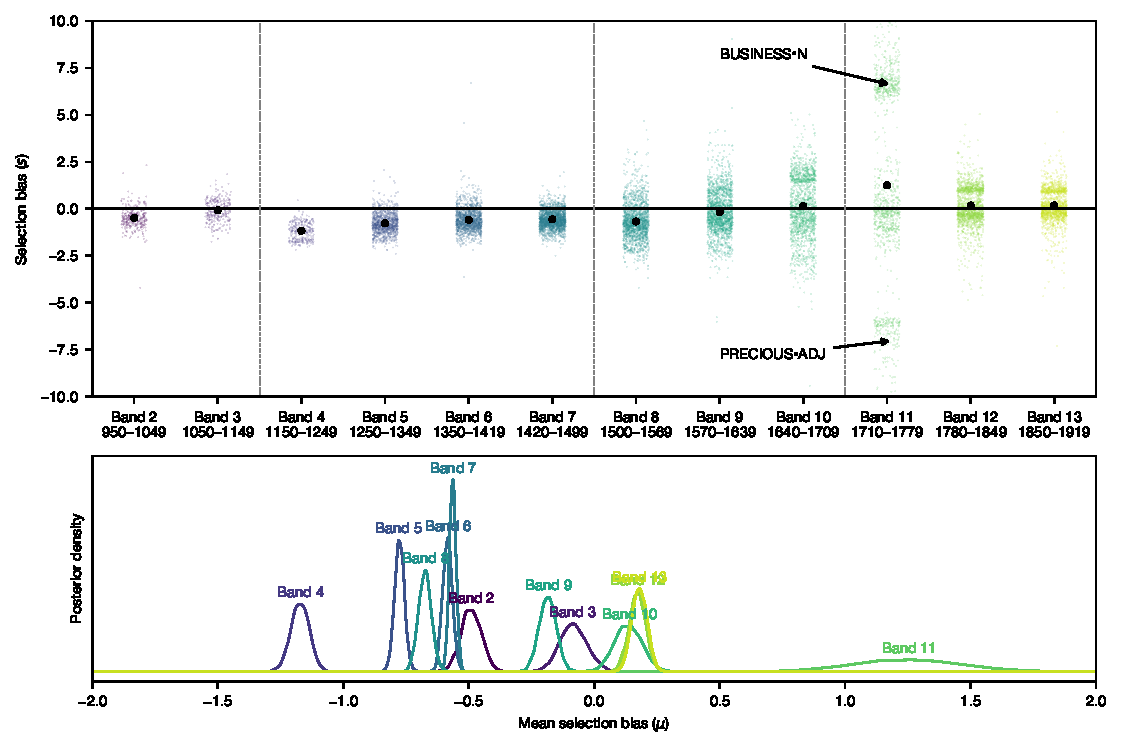
\includegraphics[]{figs/fds_posterior.pdf}}
	\vspace*{2pt}
	\caption{\textbf{\textsc{top}} Estimates of the frequency-dependent selection bias by band. Each colored dot represents an individual lemma and the black dots show the mean estimate for each band. Dashed gray lines mark the boundaries between Old, Middle, Early Modern, and Late Modern English. No results can be computed for Band~1 because this would require frequency data from a previous band. \textbf{\textsc{bottom}} Posterior estimates of the mean selection bias for each band. Bands~4 and~11 are notable outliers and show signs of a strong negative and positive frequency-dependent selection bias respectively.}
	\label{fds_posterior}
	\end{figure}

Fig.~\ref{fds_posterior} plots the results of the model. The top panel shows estimates of the frequency-dependent selection bias by band. Each colored dot represents the estimate for an individual lemma, and the black dots give the mean estimate for each band. The Old English period (Bands~2 and~3) is characterized by fairly neutral selection. This implies that the proportion with which different variants were used closely reflects their proportions at the previous timepoint, which might be explained by strong regional variation in spelling that is mostly replicated from one period to the next. The Middle English period is characterized by \textit{negative} frequency-dependent selection, particularly in Band~4. This period directly followed the Norman conquest, when English would have begun to have a lot of contact with French spelling conventions. Thus, low frequency variants (or indeed entirely new variants) would tend to be selected.

Over the Early Modern period, we see a gradual trend towards positive frequency-dependent selection, with many lemmata having estimated selection biases well above the zero line. This process seems to have culminated in Band~11, where we find not only many lemmata undergoing positive frequency-dependent selection, but also many lemmata undergoing negative frequency-dependent selection. This pattern likely stems from two major forms of change happening at this time. On the one hand, many lemmata are beginning to fix on their most common variant (positive frequency-dependent selection), while on the other, many other lemmata are switching to rare or novel variants as a wider system of spelling starts to emerge. An example for each of these categories is highlighted in the figure. In Band~11, \lemma{business}{n} has only one possible spelling, \spelling{business}, which occurs 2131 times in the corpus. This is an amplification of the previous state of affairs in Band~10, where there were four possible spellings \spelling{buisinesse} (1), \spelling{busines} (3), \spelling{business} (51), and \spelling{businesse} (3). In the case of \lemma{precious}{adj}, by comparison, the modern spelling \spelling{precious} went from being very rare in Band~10 (where \spelling{pretious} was preferred) to being the only attested spelling in Band~11.

Finally, in Bands~12 and~13, we see a reversion to neutrality. Spelling variation continues to persist in roughly the same proportions from one time point to the next, reflecting the remaining residual variation noted in the previous section.

The bottom panel in Fig.~\ref{fds_posterior} shows the posterior estimates of the by-band $\mu$ parameter of the model (i.e., the mean selection bias for each band). The estimates for Bands~10, 11, 12, and 13 are conclusively greater than zero, suggesting that, on average, lemmata were undergoing positive frequency-dependent selection at these times. It is also clear that Band~4 and Band~11 are clear outliers. One might question if the dramatic results in Band~11 are explained by the change of corpus (recall that the data for Bands~1 through~10 were taken from HCET and the data for Bands~11 through 13 were taken from CLMET). However, we found the same dramatic result when performing the analysis with the OED quotation data, suggesting that the notable effect in Fig.~\ref{fds_posterior} is not related to the change in corpus in Band~11.

%~%~%~%~%~%~%~%~%~%~%~%~%~%~%~%~%~%~%~%~%~%~%~%~%~%~%~%~%~%~%~%~%~%~%~%~%~%~%~%~%~%~%~%~%~%~%~%~%~%~%~%

\section{Discussion}

English orthography has largely been left to evolve freely across its thousand-year history. Yet modern English spelling has become standardized, even if its standardized spellings are sometimes internally inconsistent. The relative freedom with which English orthography has been allowed to evolve makes it an interesting test-case for exploring whether spelling standardization might have arisen through a process of positive frequency-dependent selection. In short, to maximize the chance of being understood, it pays for a writer to adopt spelling variants that occur with higher frequency. Ultimately, this positive frequency bias may lead to common forms becoming increasingly entrenched, and contributing to greater communicative efficiency without any guiding hand.

To evaluate this possibility, we assembled a diachronic dataset of English spelling variation, SpellEng, which we make freely available. The dataset combines the rich information on spelling variants that can be found in the \textit{Oxford English Dictionary} with a historical corpus of the English language. SpellEng tracks the variant frequencies for over 32,000 lemmata across 13 historical periods, from the earliest Old English texts to the 20th century. Although this information has existed in various forms for a long time, the SpellEng dataset brings this information together in one place to allow for the rapid exploration of how English spelling has changed over time. We pair this dataset with a mathematical model of frequency-dependent selection, allowing us to track the evolution of spelling variants over the history of the English language and classify lemmata according to whether they are undergoing positive, negative, or neutral selective forces.

Our findings suggest that English has experienced bouts of positive, negative, and neutral frequency-dependent selection through its history, but they point to the 18th century (and to a lesser extent the 17th century) as the main locus of the standardization of English spelling through the frequency-dependence mechanism. This is in broad agreement with the scholarly literature on the standardization of English spelling \parencite[e.g.,][]{Scholfield:2016}. Our observations provide the basis for thinking about the forces that give rise to periods of stability and change in English spelling. To illustrate, a large body of research in English Studies has explored the impact of socio-historical events such as the Norman Conquest and the introduction of the printing press. Our study empirically quantifies these effects, showing, for example, that the Norman Conquest led to a period of negative frequency-dependent selection, which aligns with the idea that external influences can introduce variability that may destabilize a system. Furthermore, our study's findings on the reversion to neutrality in later periods challenge the idea of a continuous progression towards standardization, highlighting how certain types of variation can become entrenched.

It is worthwhile to consider why the 18th century was such an important locus of standardization. Scholars have sometimes argued that modern spelling standardization is a social and cultural phenomenon. \textcite{Sebba:2009}, for example, argues that ``prescription'' is a product of ``the prevalent language ideology'' (p.~46), and \textcite{Cahill:2023} argues that writers first have to accept ``the very idea of standardised spelling'' (p.~151) before any such system can begin to materialize. However, we believe that there is another factor at play that motivated the drive toward standardization in the 18th century. Specifically, it was at this time that we began to see rapid growth in public literacy, and hence the ability to use written language as a principle form of communication.

Prior to the 18th century, only a small slice of the population was able to read, and reading differed substantially from its modern form. \textcite{Saenger:1997} explained that classical and medieval texts were read aloud; these texts were not consumed via the rapid, silent reading process that we know today. Likewise, \textcite{Koller:2024} argues that ancient inscriptions (particularly those with a dedicatory or memorial function) were sometimes not meant to be read at all. In the absence of pressure to process large amounts of text at speed, there is really no need for standardization. Likewise, our analysis shows that in the Old and Middle English periods, spelling was characterized largely by negative frequency-dependent selection, with rare variants being used and new variants being attested. There was probably also an overarching practice of writing words as they sound; spellings may thus reflect individual author dialects as well as diachronic sound change.

The advent of public literacy in the 18th century changed the picture substantially. Because texts were being shared much more widely across a larger group of readers, there would increasingly have been pressure for standardization to ensure that writers were understood. This pressure for standardization may also have led to the conservation of high-frequency spellings following a sound change (e.g., the conservation of spellings like \spelling{which} despite the loss of the \pronunciation{w}--\pronunciation{ʍ} distinction); this may account for some of the idiosyncrasy of English spelling \parencite[see][for discussion]{Berg:2021, CarrRastle:2024}. The 18th century probably also saw an increasing pressure for reading efficiency. Reading by this point had become a rapid, silent activity requiring a high degree of skill; in fact, analysis of contemporary silent reading speeds suggests an average of 238 words per minute \parencite{Brysbaert:2019}. Research also indicates that modern text tends to communicate far more information (in terms of vocabulary density and syntactic complexity) than spoken language \parencite{Nation:2022}. Thus, readers in the 18th century would have increasingly needed to consume large amounts of information at speed, and that information would have originated from different parts of the country (or even the world).

Even under these circumstances, one might argue that it should be possible to cope with spelling variation as long as the spellings being used are transparently related to the intended spoken words. Thus, the use of spellings such as \spelling{brane}, \spelling{brain}, \spelling{brayn}, \spelling{brayne}, \spelling{braen}, and \spelling{braene} might all function to get to the intended meaning of the organ in one's head. However, a story written by the second author's daughter (at the age of five) demonstrates why this type of system could never support rapid, skilled reading:
\begin{quote}
Wunse ther was a piroote he was cald timbers his croo was loud and nastee timbers was the captin his croo saled to a desert they dug up some tresher the end
\end{quote}
It is possible to read and understand this story but trying to decode the unfamiliar spellings slows the reader down. Indeed, psychological research on reading suggests that readers essentially learn to memorize the orthographic forms of words over the long period of reading acquisition \parencite[a process called ``orthographic learning'';][]{Castles:2006}, and this allows their meanings to be retrieved especially rapidly. If spellings regularly change over time and differ between speakers because of a lack of standardization, then this rapid retrieval process cannot occur.

This analysis suggests that the standardization of English spelling was intimately tied to the rise of public literacy. The sheer number of people from different regions producing and consuming text required use of a standard set of spellings---although whether rising public literacy resulted from standardization or the reverse remains to be investigated. Yet, one question that we haven't addressed is why the standardization process resulted in such a non-optimal set of spellings. The notion of frequency-dependent selection may provide an answer if we assume that the selection process operates at the level of the whole word as opposed to the grapheme. The cultural evolution of spelling settles on the highest-frequency variant of a whole word to maximize communicative efficiency, but this sometimes leads to internal inconsistencies that are non-optimal for learning.

% For example, it is around the end of the 17th century that we see the emergence of a distinct letter \spelling{j} (derived from \spelling{i}) for marking consonants (\spelling{iealousie} → \spelling{jealousy}) and the specialization of \spelling{u} and \spelling{v} (originally the same letter) for vowels and consonants respectively (\spelling{loue} → \spelling{love}, \spelling{vggly} → \spelling{ugly}) \parencite{CondorelliUVIJ:2021}.

Our work in this article has provided new theoretical insights into the way that linguistic dynamics and historical events have contributed to stability and change in the past 1000 years of English spelling. However, our work also provides an important set of methodological advances. We have shown how a mathematical model can be applied to historical linguistic data to infer the nature of selection biases over time. Future research could build on this approach by exploring other linguistic phenomena, such as syntactic or lexical changes, or standardization processes across different languages. Our development and open release of the SpellEng diachronic dataset will also facilitate the work of other research groups interested in English spellings across the past 1000 years. For example, analyses like that of \textcite{CondorelliUVIJ:2021} on the distributions of \spelling{u}/\spelling{v} and \spelling{i}/\spelling{j} can be performed quite easily by extracting the relevant words and tracing the proportions over time. Similarly, the diachronic analysis of \textcite{Berg:2017} can be replicated by extracting all lemmata with a given suffix (e.g., \textsc{-ness}) and calculating the usage proportions of different spellings (\spelling{-nes}, \spelling{-nesse}, \spelling{-nis}, etc.). The dataset could also be used in a data-driven way to flag up interesting spelling changes that may not have been previously recognized. For example, by extracting and comparing the dominant forms from consecutive bands, one may perhaps be able to discover interesting patterns such as a shift to \spelling{c}-final spellings in \pronunciation{k}-final nouns (e.g., \spelling{magick} → \spelling{magic}, \spelling{republick} → \spelling{republic}, \spelling{zodiack} → \spelling{zodiac}) and \spelling{ck}-final spellings in \pronunciation{k}-final verbs (e.g., \spelling{blok} → \spelling{block}, \spelling{lac} → \spelling{lack}, \spelling{smacke} → \spelling{smack}).

Overall, we suggest that the standardized irregularity of English spelling might be explained through the evolutionary process of frequency-dependent selection. In the absence of careful top-down reform of the orthographic system, the spellings of English words (and morphemes) largely standardized on whatever form happened to be most frequent around the 17th and 18th centuries. Importantly, we suggest that this process occurred due to the communicative advantage of aligning on a single spelling in the context of an emerging literate society. We support this analysis with a mathematical model of frequency-dependent selection fit to corpus data on the relative proportions with which different spelling variants were in use across one thousand years. By quantifying how spelling variants change over time, it is our hope that the SpellEng dataset may prove useful in future analyses of English orthography and in the cultural evolution of language more generally.

%~%~%~%~%~%~%~%~%~%~%~%~%~%~%~%~%~%~%~%~%~%~%~%~%~%~%~%~%~%~%~%~%~%~%~%~%~%~%~%~%~%~%~%~%~%~%~%~%~%~%~%

\section{Acknowledgments}

\noindent This work was funded by a Leverhulme Trust Research Project Grant awarded to KR (grant number: RPG-2020-034). We are grateful to Aaron Koller for valuable discussion.

\printbibliography

\end{document}